\bexo
Tracer sur la même figure
\begin{itemize}
	\item $x\mapsto 2x^2$
	\item $x\mapsto 2(x+1)^2$
	\item $x\mapsto 2(-x-1)^2$
	\item $x\mapsto 2(-x+1)^2$
\end{itemize}
\eexo
\solution{
Les graphes des fonctions sont:\\
\begin{center}
	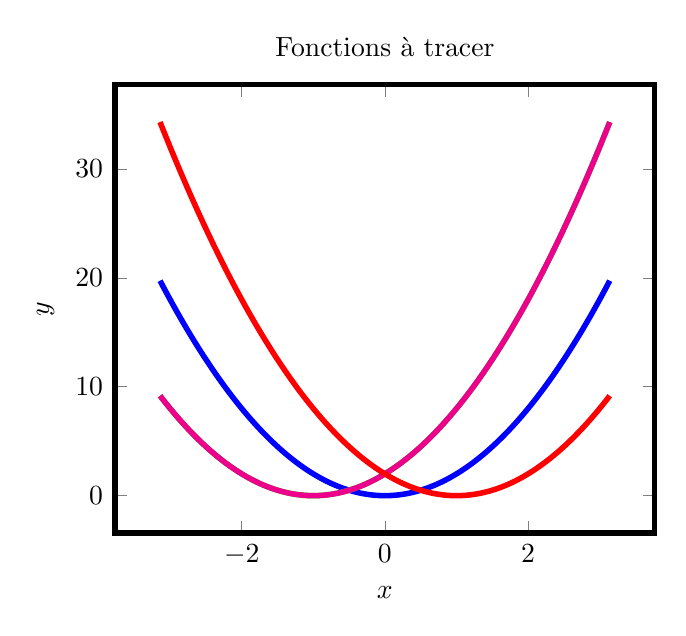
\begin{tikzpicture}
	  \begin{axis}[line width=2pt,       legend columns=-1,
   title=Fonctions à tracer,
   xlabel={$x$},
   ylabel={$y$}, legend entries={$2x^2$,$2(x+1)^2$,$2(-x-1)^2$,$2(-x+1)^2$},
	  legend to name=named]
		\addplot[blue] expression[domain=-pi:pi,samples=500]{2*x^2};
		\addplot[green,samples=500] expression[domain=-pi:pi]{2*(x+1)^2};
		\addplot[magenta,samples=500] expression[domain=-pi:pi]{2*(x+1)^2};
		\addplot[red,samples=500] expression[domain=-pi:pi]{2*(x-1)^2};				
	  \end{axis}

	\end{tikzpicture}
		  \ref{named}
\end{center}
}
